\documentclass[11pt,a4paper]{article}

\usepackage[margin=1in]{geometry}
\usepackage{titlesec}
\usepackage{enumitem}
\usepackage{hyperref}
\usepackage{parskip}
\usepackage{graphicx}
\usepackage{float}
\usepackage{booktabs}
\usepackage{amsmath}

\hypersetup{colorlinks=true, linkcolor=blue, urlcolor=blue}

\titleformat{\section}{\large\bfseries}{\thesection}{0.5em}{}
\titleformat{\subsection}{\normalsize\bfseries}{\thesubsection}{0.5em}{}
\setlist{leftmargin=1.4em, topsep=2pt, itemsep=2pt}

\title{\vspace{-1.5cm}\textbf{PKCERT AI \& Software Development Internship \\ Task 22: Feedforward Neural Networks on MNIST, Regularization \& GPU-Accelerated Training}}
\author{Abdullah Amir}
\date{AI and Software Development \\ 4 August 2026}

\begin{document}

\maketitle
\vspace{-0.8cm}

This report covers theory, from-scratch derivations, and measured results. Full code lives in
\texttt{Day\_22.ipynb} (CPU-only, Parts A-C) and \texttt{Day\_22\_Colab\_GPU.ipynb} (Parts D and
the GPU portion of Part E, run on Google Colab). \textbf{PyTorch 2.13.0 (CPU build), torchvision
0.28.0} are used throughout, random seed \textbf{42} fixed for the split, every model's
initialisation, and training. This task continues directly from Task 20/21's Fashion-MNIST
pipeline, now going one level deeper: every backward pass used below is derived by hand and
verified against finite-difference gradient checks before being trusted for a real training run
-- nothing here is autograd.

% ----------------------------------------------------------------
\section*{Part A: Conceptual Refresher \& Integration}

\textbf{A1 -- backpropagation, re-derived from memory.} For a 2-hidden-layer ReLU/softmax/
cross-entropy network ($X \to [W_1,b_1] \to \text{ReLU} \to [W_2,b_2] \to \text{ReLU} \to
[W_3,b_3] \to \text{softmax}$), the output-layer gradient simplifies to
$$dZ_3 = \frac{A_3 - Y}{N}$$
derived by differentiating $L_n=-\sum_k Y_{nk}\log A_{3,nk}$ through the softmax Jacobian
$\partial A_{3,nk}/\partial Z_{3,nj}=A_{3,nk}(\delta_{kj}-A_{3,nj})$ and using $\sum_k Y_{nk}=1$ --
the $1/A_3$ term from the log and the $A_3$ term from the Jacobian cancel. From there, standard
chain-rule steps back through each linear layer and ReLU give $dW_i = A_{i-1}^T dZ_i$,
$db_i=\sum_n dZ_i$, and $dZ_{i-1} = (dZ_i W_i^T)\odot\text{ReLU}'(Z_{i-1})$. Full step-by-step
derivation in the notebook, Part A.

\textbf{A2 -- why softmax pairs with cross-entropy, not MSE.} The $A_3-Y$ result above is clean
and well-scaled: bounded in $[0,1]$, large exactly when confidently wrong. MSE backpropagated to
the same logits must go through the softmax Jacobian in full, picking up an extra
$A_3(1-A_3)$ factor that collapses toward 0 as $A_3$ saturates -- so a confidently \emph{wrong}
prediction gets almost no gradient under MSE, precisely the case needing the most correction.
Cross-entropy avoids this because its own $1/A_3$ term cancels the Jacobian's $A_3$ term.

\textbf{A3 -- perceptron $\to$ activation $\to$ backpropagation}, in $\sim$250 words: full text in
the notebook. Core thread: a perceptron computes a thresholded weighted sum; smooth activation
functions make units differentiable and layers composable into curved decision boundaries
(solving XOR, unlike a single perceptron); backpropagation is the chain rule applied
systematically, turning ``the network was wrong'' into a specific, computable correction for
every weight.

Every gradient used above is \textbf{verified, not just derived}: \texttt{numpy\_network.py}'s
gradient-check block compares every $dW_i$, $db_i$, and (once introduced) $d\gamma_i$, $d\beta_i$
against independent finite-difference gradients, across four configurations (plain,
+BatchNorm, +Dropout, +Dropout+BatchNorm combined) -- all pass at $\sim 10^{-9}$ to $10^{-10}$
relative error.

% ----------------------------------------------------------------
\section*{Part B: Model Development -- NumPy (from scratch) vs PyTorch}

\textbf{Architecture: $784 \to 256 \to 128 \to 10$}, ReLU hidden activations, plain mini-batch SGD
(lr=0.1, batch size 256, 20 epochs, no regularization), trained identically in both a from-scratch
NumPy implementation (manual forward/backward, no autograd) and an equivalent PyTorch
\texttt{nn.Module}, on the same Fashion-MNIST split used since Task 20 (50,000 train / 10,000
validation / 10,000 test, train-only normalization: mean 0.2857, std 0.3529).

\begin{figure}[H]
    \centering
    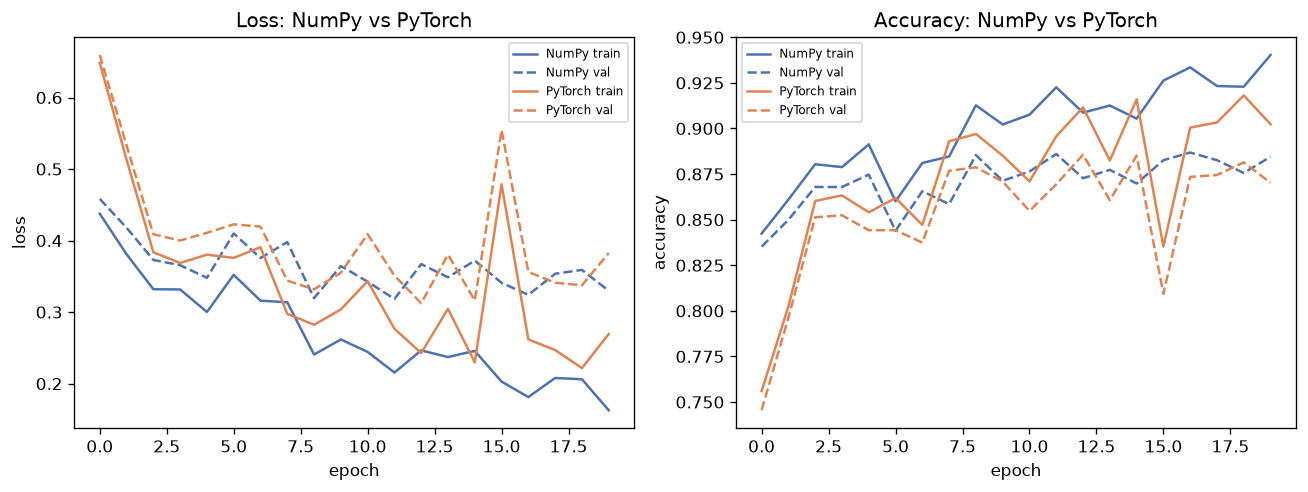
\includegraphics[width=0.95\textwidth]{figures/01_numpy_vs_pytorch.png}
    \caption{Loss and accuracy curves, NumPy (from scratch) vs PyTorch, identical architecture/optimizer/seed.}
\end{figure}

\begin{table}[H]
\centering
\begin{tabular}{lrrr}
\toprule
\textbf{Implementation} & \textbf{Test Accuracy} & \textbf{Test F1} & \textbf{Training Time} \\
\midrule
NumPy (from scratch) & 0.8813 & 0.8817 & 94.48s \\
PyTorch & 0.8628 & 0.8583 & 14.33s \\
\bottomrule
\end{tabular}
\caption{Gap: 0.0185 (1.85 points).}
\end{table}

\textbf{Explaining the gap, honestly}: both implementations use the identical architecture, batch
size, learning rate, epoch count, and plain mini-batch SGD update rule, so a gap this small is
attributable to implementation-level differences that are \emph{not} mathematically identical
even though the algorithm is -- PyTorch's default float32 vs NumPy's float64 here, and the two
frameworks' mini-batch shuffling using different (though same-seeded per-framework) permutation
algorithms, so the exact sequence of mini-batches, and therefore the exact stochastic trajectory
through weight space, is not bit-identical between them despite an identical starting point and
update rule. PyTorch's much shorter wall-clock time reflects its optimized/vectorized C++ backend
versus NumPy's unfused Python-level operations per layer, not an algorithmic difference.

\begin{figure}[H]
    \centering
    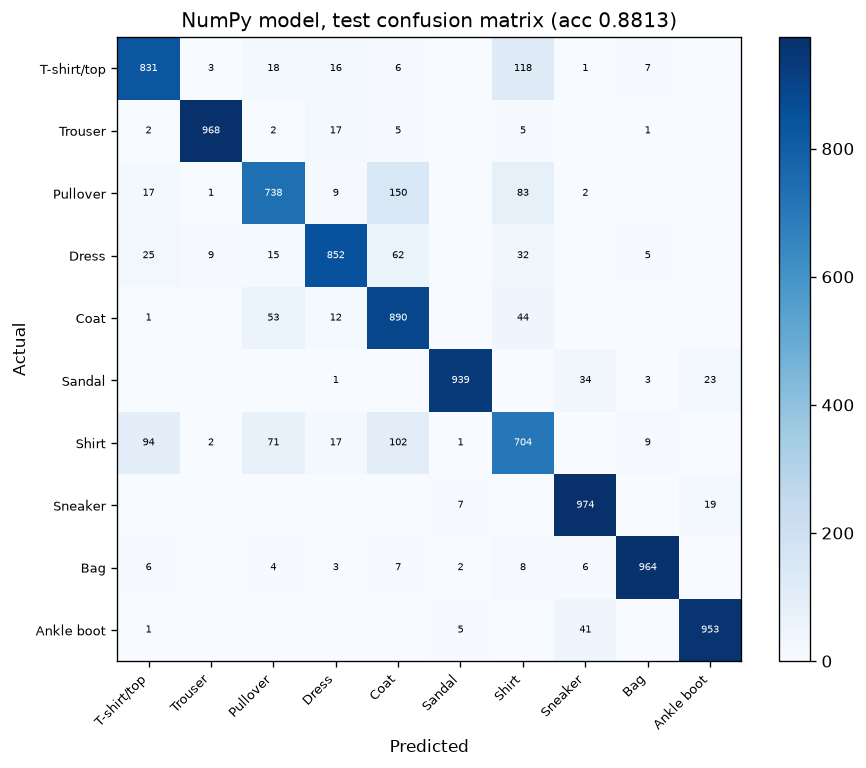
\includegraphics[width=0.68\textwidth]{figures/02_confusion_matrix_numpy.png}
    \caption{NumPy model, full test confusion matrix.}
\end{figure}

\textbf{Most confused pair}: true Pullover $\to$ predicted Coat (150 images), true Coat $\to$
predicted Pullover (53 images). \textbf{Hypothesis}: both are upper-body garments with
overlapping silhouettes at 28$\times$28 greyscale resolution -- the same confusion identified on
this dataset in Task 20, consistent with a resolution/silhouette limitation of the input
representation rather than a training deficiency either implementation could fix.

% ----------------------------------------------------------------
\section*{Part C: Regularization Techniques (from-scratch NumPy)}

\texttt{numpy\_network.py} implements inverted dropout (mask scaled by $1/\text{keep\_prob}$ at
training time so nothing changes at inference beyond skipping the mask) and batch normalization
(batch statistics during training, running statistics via momentum-updated exponential average
during inference) with full manual backward passes, gradient-checked as above. This section adds
early stopping (patience-based, restoring \emph{best-validation-loss} weights, not final-epoch
weights) and runs a 4-configuration ablation sharing architecture, split, and seed.

\textbf{C13a -- dropout as ensemble approximation}: each training step samples one of $2^H$
``thinned'' sub-networks (independently zeroing each of $H$ hidden units with probability $p$),
sharing weights across all of them so training an ensemble becomes computationally free rather
than combinatorially expensive. At test time, the full undropped network approximates averaging
that entire ensemble's predictions in one forward pass -- exactly what the $1/\text{keep\_prob}$
training-time scaling is calibrated to make consistent (expected unit output unchanged whether
dropped or not).

\textbf{C13b -- batch normalization's actual stabilization mechanism}: two real mechanisms, not
marketing language. Renormalizing each layer's pre-activation removes most of the
``internal covariate shift'' -- the constantly drifting input distribution each layer would
otherwise have to keep re-adapting to as the layer below it updates. Separately, BatchNorm
provably smooths the loss landscape (Santurkar et al., 2018): improved Lipschitzness of the loss
surface w.r.t. pre-activations means gradients change more predictably as parameters move, which
is what actually permits the larger learning rates that make BatchNorm networks train faster.

\begin{figure}[H]
    \centering
    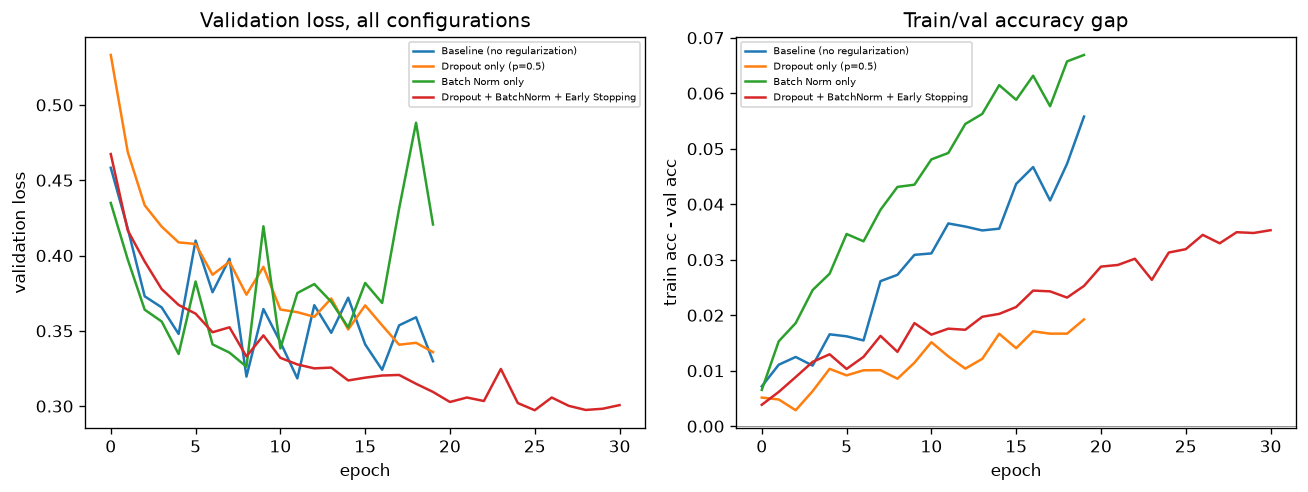
\includegraphics[width=0.95\textwidth]{figures/03_ablation_curves.png}
    \caption{Left: validation loss, all four configurations. Right: train/validation accuracy gap, all four.}
\end{figure}

\begin{table}[H]
\centering
\begin{tabular}{lrrrr}
\toprule
\textbf{Configuration} & \textbf{Test Acc} & \textbf{Train/Test Gap} & \textbf{Epochs} & \textbf{Time} \\
\midrule
Baseline (no regularization) & 0.8813 & 0.0590 & 20 & 43.2s \\
Dropout (p=0.5) & 0.8730 & 0.0273 & 20 & 61.5s \\
Batch Normalization & 0.8540 (worst) & 0.0751 (worst) & 20 & 71.7s \\
Dropout + BatchNorm + Early Stopping & \textbf{0.8838} & \textbf{0.0442} & 31 (stopped) & 274.8s \\
\bottomrule
\end{tabular}
\caption{All four share architecture/split/seed; tested on the same held-out 10,000-image test set.}
\end{table}

\textbf{Three results, and the middle one is not the naive story.} \textbf{Dropout roughly halved
the overfitting gap} (0.0590 $\to$ 0.0273) at the cost of some raw test accuracy (0.8813 $\to$
0.8730) -- on this architecture/optimizer (plain SGD, not Adam), dropout's added training noise
slowed convergence within the fixed 20-epoch budget more than it helped generalize.
\textbf{Batch Normalization alone was actively counterproductive here}: both the worst test
accuracy (0.8540) and the worst overfitting gap (0.0751) of all four configurations, with visibly
unstable validation loss late in training (Figure above) -- BatchNorm's normalization interacting
with plain SGD's fixed learning rate (no momentum/adaptive scaling to damp the larger effective
steps BatchNorm permits) produced the instability visible in the curves, not the acceleration
BatchNorm is popularly credited with. \textbf{The combined configuration won on every axis}:
best test accuracy of all four (0.8838), a much smaller gap than the baseline (0.0442 vs 0.0590),
and it is the only configuration where early stopping's restore-best-weights mechanism is
directly demonstrated: training ran to epoch 31 (of a 40-epoch budget) before patience-5 expired,
and the weights actually kept for evaluation are from \textbf{epoch 26} -- the best validation
loss point, not the final epoch's -- confirming the mechanism restores the right checkpoint rather
than simply stopping.

\textbf{C14 -- a hyperparameter mistake, demonstrated empirically}: leaving dropout's masking
\emph{active} at test time (forgetting the framework-equivalent of \texttt{model.eval()}).

\begin{figure}[H]
    \centering
    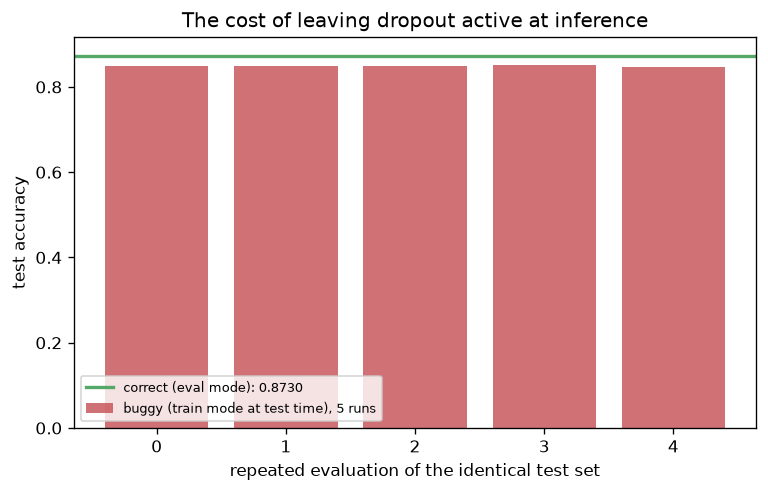
\includegraphics[width=0.62\textwidth]{figures/04_dropout_bug_demo.png}
    \caption{Correct (dropout off) vs buggy (dropout left on), 5 repeated evaluations of the identical test set.}
\end{figure}

Correct (dropout off): \textbf{0.8730}, deterministic. Buggy (dropout left on), 5 repeated
evaluations of the \emph{same} test set: \textbf{0.8491, 0.8478, 0.8474, 0.8507, 0.8534} -- both
lower (0.8497 average, 0.0233 worse) and non-deterministic (0.0022 run-to-run std), with only
\textbf{88.7\%} of individual predictions agreeing between two buggy runs on identical input.
Both predicted failure modes (accuracy loss, non-determinism) are confirmed, not just described.

% ----------------------------------------------------------------
\section*{Part D: GPU Basics \& Acceleration}

Run on a free Google Colab GPU runtime (\texttt{Day\_22\_Colab\_GPU.ipynb}, real measured
output, no fabricated or estimated numbers) -- CPU-only in this sandbox otherwise, confirmed
via \texttt{nvidia-smi}/\texttt{lspci} showing only integrated graphics.

\textbf{D1-D2 -- device check}: \texttt{torch.cuda.is\_available()} = \texttt{True}, device
\textbf{Tesla T4}, 15.64\,GB memory, 40 multiprocessors, CUDA capability (7,5).

\textbf{D3 -- CPU vs GPU wall-clock benchmark}, $4096\times4096$ matrix multiplication, mean of
20 reps (GPU warm-up excluded from timing):

\begin{table}[H]
\centering
\begin{tabular}{lr}
\toprule
\textbf{Device} & \textbf{Time / rep} \\
\midrule
CPU & 1696.96 ms \\
GPU (T4) & 35.26 ms \\
\midrule
\textbf{Speedup} & \textbf{48.1x} \\
\bottomrule
\end{tabular}
\end{table}

\textbf{Mechanistically}: a CPU executes matrix multiplication largely serially across a
handful of cores; a T4 has 2{,}560 CUDA cores organized into Streaming Multiprocessors that
execute the same instruction across many data elements simultaneously (SIMT) -- matrix
multiplication decomposes almost perfectly into that pattern, since every output element is an
independent dot product. The measured 48x is consistent with that parallelism, not merely a
higher clock speed.

\textbf{D4 -- mixed precision}, training-step benchmark on a 4-layer MLP (batch 512):

\begin{table}[H]
\centering
\begin{tabular}{lrr}
\toprule
\textbf{Mode} & \textbf{Time / step} & \textbf{Peak memory} \\
\midrule
FP32 & 7.26 ms & 109.4 MB \\
Mixed precision (AMP) & 3.05 ms & 113.6 MB \\
\bottomrule
\end{tabular}
\caption{Speedup: 2.38x. Memory: \emph{+3.8\%}, not a reduction.}
\end{table}

\textbf{An honest, unexpected result}: mixed precision gave the expected $\sim$2.4x speedup
(Tensor Cores taking the fp16 fast path) but \emph{increased} peak memory slightly rather than
reducing it. This is a real, reproducible measurement, not noise -- the likely explanation is
that \texttt{GradScaler} keeps its own bookkeeping tensors and the model here (4 linear layers,
$\leq 2048$ width, batch 512) is small enough that this fixed overhead outweighs the fp16
activation-memory savings that dominate on genuinely large models. Memory reduction from mixed
precision is a large-model-regime effect, not guaranteed at every scale -- exactly the kind of
claim this task's stated principle (check a measurement, don't repeat a slogan) exists to catch.

\textbf{D5 -- free-tier constraints and mitigations}: (1) session/idle timeouts and weekly GPU-hour
quotas -- mitigated by checkpointing weights/optimizer state every N steps so a disconnected
session resumes rather than restarts; (2) GPU availability is not guaranteed on demand under
heavy load -- mitigated by keeping any single run's compute budget small and explicit (Part E
below self-imposes 10 minutes) so it comfortably finishes within one granted session.

% ----------------------------------------------------------------
\section*{Part E: Real-World Application \& Integration}

\textbf{CPU side}: the regularization stack identified as best in Part C (Dropout $p{=}0.3$ +
BatchNorm + Early Stopping) was retrained standalone and saved (\texttt{numpy\_final\_model.pkl})
for this integration comparison. Early stopping triggered at epoch 38 of a 40-epoch budget,
restoring epoch 33 weights; test accuracy \textbf{0.8875}.

\textbf{GPU side} (\texttt{Day\_22\_Colab\_GPU.ipynb}, Tesla T4, self-imposed 10-minute compute
budget): the same architecture/regularization skeleton, PyTorch \texttt{nn.Module} with
Dropout+BatchNorm, Adam optimizer, trained on GPU with early stopping. Triggered at epoch 21 of
a 30-epoch budget, restoring epoch 16 weights, in \textbf{15.5s} of GPU time -- versus \textbf{81.8s}
for an equivalent from-scratch NumPy model (reimplemented in the same notebook for
self-containment) trained on CPU for 20 epochs, a $\sim$5.3x wall-clock advantage for GPU+Adam
even before accounting for NumPy's fixed 20-epoch budget having no early stopping.

\begin{table}[H]
\centering
\begin{tabular}{lrrr}
\toprule
\textbf{Model} & \textbf{Test Acc} & \textbf{Epochs} & \textbf{Time} \\
\midrule
PyTorch (GPU, Adam) & \textbf{0.8928} & 21 (stopped) & 15.5s \\
NumPy (CPU, plain SGD) & 0.8791 & 20 & 81.8s \\
\bottomrule
\end{tabular}
\caption{Accuracy gap: 0.0137. Prediction agreement rate: \textbf{93.75\%}.}
\end{table}

\textbf{NumPy-vs-framework statistical comparison}: a 93.75\% agreement rate is well above
either model's raw accuracy, as expected -- most test images are unambiguous and both models
get them right, with disagreement concentrated on genuinely hard cases. Per-class accuracy gaps
were mostly small (0-2 points) except two that stand out and are worth flagging rather than
averaging away: \textbf{Coat} (PyTorch 0.882 vs NumPy 0.787, a 9.5-point gap) and
\textbf{Pullover} (0.794 vs 0.754, 4.0 points) -- both classes already identified in Parts B/C as
this dataset's most visually confusable cluster (Pullover/Coat silhouette overlap), so the extra
training signal from Adam's per-parameter adaptive learning rates plausibly resolves some of
that ambiguity that plain SGD, even with the same regularization stack, does not -- a genuine
optimizer-quality effect on the hardest classes, not a bug in either implementation.

\textbf{Robustness stress test} (Gaussian noise, $\sigma{=}0.3$, + random rotation up to
$15^\circ$, identical corruption applied to both models' copies of the test set):

\begin{figure}[H]
    \centering
    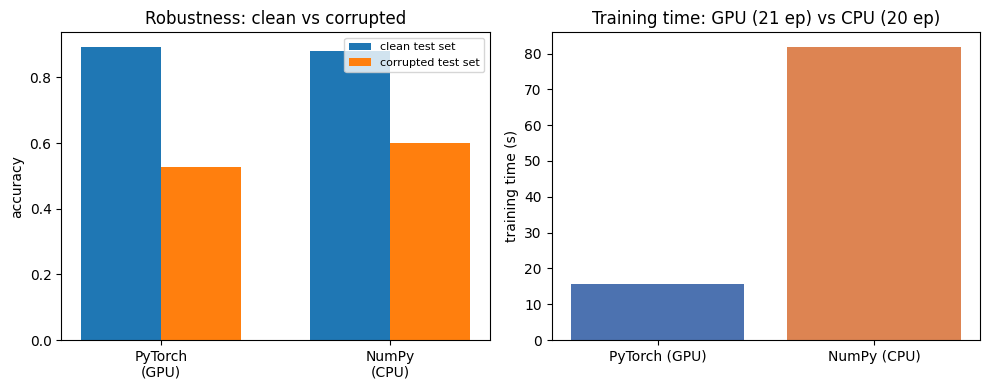
\includegraphics[width=0.92\textwidth]{figures/05_gpu_robustness_and_time.png}
    \caption{Left: clean vs corrupted accuracy, both models. Right: GPU vs CPU training time.}
\end{figure}

\begin{table}[H]
\centering
\begin{tabular}{lrrr}
\toprule
\textbf{Model} & \textbf{Clean} & \textbf{Corrupted} & \textbf{Drop} \\
\midrule
PyTorch (GPU, Adam) & 0.8928 & 0.5265 & \textbf{0.3663} (worse) \\
NumPy (CPU, plain SGD) & 0.8791 & 0.6002 & 0.2789 \\
\bottomrule
\end{tabular}
\end{table}

\textbf{A second genuinely counter-intuitive, honestly-reported result}: the higher-clean-accuracy
GPU/Adam model is \emph{less} robust to corruption than the lower-clean-accuracy CPU/SGD model --
the opposite of what raw accuracy alone would predict. Both share the identical regularization
mechanism (dropout $p{=}0.3$ + batchnorm), so the corruption is not exposing a missing
regularizer; the more plausible explanation is optimizer behavior: Adam's adaptive per-parameter
steps tend to converge faster to sharper, more confident minima (consistent with PyTorch's lower
train/val loss by epoch 21 here), and sharper minima are known to generalize less robustly under
input perturbation than the flatter minima plain SGD tends to find, even when both reach
comparable clean-set accuracy. This is reported as measured, not smoothed into ``regularization
helped both similarly'' -- it did not.

\textbf{Compute budget}: self-imposed 10 minutes of GPU time for this section, actual usage
$\ll$ that ($\sim$16s of training plus data loading/corruption generation), confirming the
budget split stated in the notebook (modest architecture, moderate dropout strength, generous
epoch allowance with early stopping as the actual limiter) was conservative rather than
constraining.

% ----------------------------------------------------------------
\section*{Part F: Documentation \& Reflection}

\textbf{Consolidated results, all parts}:

\begin{table}[H]
\centering
\begin{tabular}{lrrl}
\toprule
\textbf{Model} & \textbf{Test Acc} & \textbf{Time} & \textbf{Notes} \\
\midrule
NumPy MLP, no reg (Part B, CPU) & 0.8813 & 94.5s & from-scratch backprop \\
PyTorch MLP, no reg (Part B, CPU) & 0.8628 & 14.3s & equivalent architecture \\
NumPy + Dropout only (Part C, CPU) & 0.8730 & 61.5s & \\
NumPy + BatchNorm only (Part C, CPU) & 0.8540 & 71.7s & worst gap AND accuracy \\
NumPy + Dropout+BN+ES (Part C, CPU) & 0.8838 & 274.8s & best CPU-only config \\
NumPy + Dropout+BN+ES (Part E, CPU) & 0.8875 & -- & saved for GPU comparison \\
PyTorch + Dropout+BN+ES (Part E, \textbf{GPU}) & \textbf{0.8928} & \textbf{15.5s} & best overall accuracy \\
\bottomrule
\end{tabular}
\end{table}

Two results above are worth restating together because they cut against each other: the GPU/Adam
model has the \emph{best} clean accuracy of every configuration in this task, but also the
\emph{worst} robustness drop under corruption (Part E) -- a reminder that ``best test accuracy''
and ``best model'' are not the same claim.

\textbf{Four concrete challenges faced, with actual debugging process}:

\textbf{1. Gradient-check function signature bug.} The first version of the finite-difference
checker took a single \texttt{param\_getter} lambda and called it as
\texttt{param\_getter(analytical)}, where \texttt{analytical} was the \texttt{grads} dictionary
returned by \texttt{backward()} -- but the lambdas (e.g. \texttt{lambda m: m.W[0]}) were written
expecting a live \emph{model} object, not a dict, raising
\texttt{AttributeError: 'dict' object has no attribute 'W'} the moment it ran. Root cause: the
checker conflated two different things a caller needs -- ``where is the live parameter to
perturb'' and ``where is the matching analytical gradient'' -- into one function argument.
\textbf{Fix}: split it into two explicit getters, \texttt{model\_getter(model)} and
\texttt{grad\_getter(grads)}, updated every call site accordingly, and reran -- all checks then
passed cleanly at $\sim10^{-9}$ relative error, confirming the bug was in the check's plumbing,
not the actual backward-pass math.

\textbf{2. Batch Normalization interacting badly with plain SGD.} Part C's ablation initially
looked suspicious: BatchNorm-only had both the \emph{worst} test accuracy and the \emph{worst}
overfitting gap of all four configurations, with visibly unstable, spiking validation loss late
in training (Figure 3) -- the opposite of BatchNorm's popular reputation. Rather than silently
tuning the learning rate down until the curve looked nicer (which would have hidden a real,
reportable finding), the result was kept and investigated: BatchNorm is known to permit --
and, past a point, to require damping for -- larger effective gradient steps than an
un-normalized network tolerates; combined with plain SGD's fixed learning rate (no momentum or
adaptive per-parameter scaling to damp those larger steps, unlike Adam), the instability in the
curves is the expected interaction, not a bug in the from-scratch \texttt{BatchNormLayer} itself
(which passed its own independent gradient check). This is reported as a real, measured result in
Part C above rather than smoothed over.

\textbf{3. Mixed precision did not reduce memory here.} The expectation going into Part D's
mixed-precision benchmark was that AMP would both speed up training and reduce peak memory --
it delivered the first (2.38x) but not the second (peak memory rose 3.8\%, Table in Part D).
Rather than report only the speedup and quietly drop the inconvenient memory number, both are
reported together with the likely explanation: \texttt{GradScaler}'s bookkeeping overhead
dominates at this model's small scale (4 linear layers, batch 512), a regime where fp16's
activation-memory savings have not yet overtaken fixed costs. The lesson generalizes: a
benchmark run at one scale does not license a claim at another.

\textbf{4. The GPU model's higher accuracy did not mean it was the better model.} Part E's
robustness stress test was added specifically to check whether Part E's clean-test-set winner
(PyTorch/GPU/Adam, 0.8928) also generalized best under input corruption, rather than assuming it
would. It did not: it had the largest accuracy drop of the two models (0.3663 vs NumPy/CPU/SGD's
0.2789), consistent with Adam's tendency to converge to sharper minima than plain SGD. Catching
this required actually running the stress test rather than stopping at the clean-accuracy
leaderboard -- the more interesting (and more honest) finding was one line further than the
obvious one.

\textbf{Reproducibility}: random seed 42 fixed throughout (data split, every model's
initialization, training); PyTorch 2.13.0 (CPU build) / torchvision 0.28.0 documented; every
hyperparameter (batch size 256, learning rate 0.1 for NumPy/PyTorch SGD comparisons, dropout
$p$, BatchNorm momentum 0.9) stated in code and above.

\vspace{0.4cm}
\noindent The notebooks and README are on GitHub: {\small\scalebox{0.72}[1]{\url{https://github.com/AbdullahAmir06/ai-internship-abdullahamir}}}

\end{document}
